\begin{section}{Resultados}
	El siguiente gráfico se realizó para ajustar un parámetro ($epsilon$) del programa que sirve para generar las matrices mal condicionadas. Recordar que la matriz se construye a partir de un vector que resulta en las filas de la misma y luego se le suma el $epsilon$ a los elementos de la diagonal para que quede inversible.
	
	Con esta prueba esperamos ver que cuanto menor es el $epsilon$ mayor es el número de condición de la matriz debido a que las filas están más cerca de ser linealmente dependientes y por ende la matriz más cerca de ser singular.

	Se graficó el número de condición de la matriz en función de su dimensión para los siguientes valores de $epsilon$: $1$, $1e^{-1}$, $1e^{-2}$, $1e^{-3}$, $1e^{-4}$, $1e^{-5}$ y $1e^{-6}$. Corrimos las pruebas para matrices de dimensión $2$ a dimensión $50$.
	El eje que corresponde al \texttt{número de condición} está en escala logarítmica para poder apreciar mejor los valores correspondientes dado que estos crecen exponencialmente.

	\begin{figure}[H]
	  \centering
		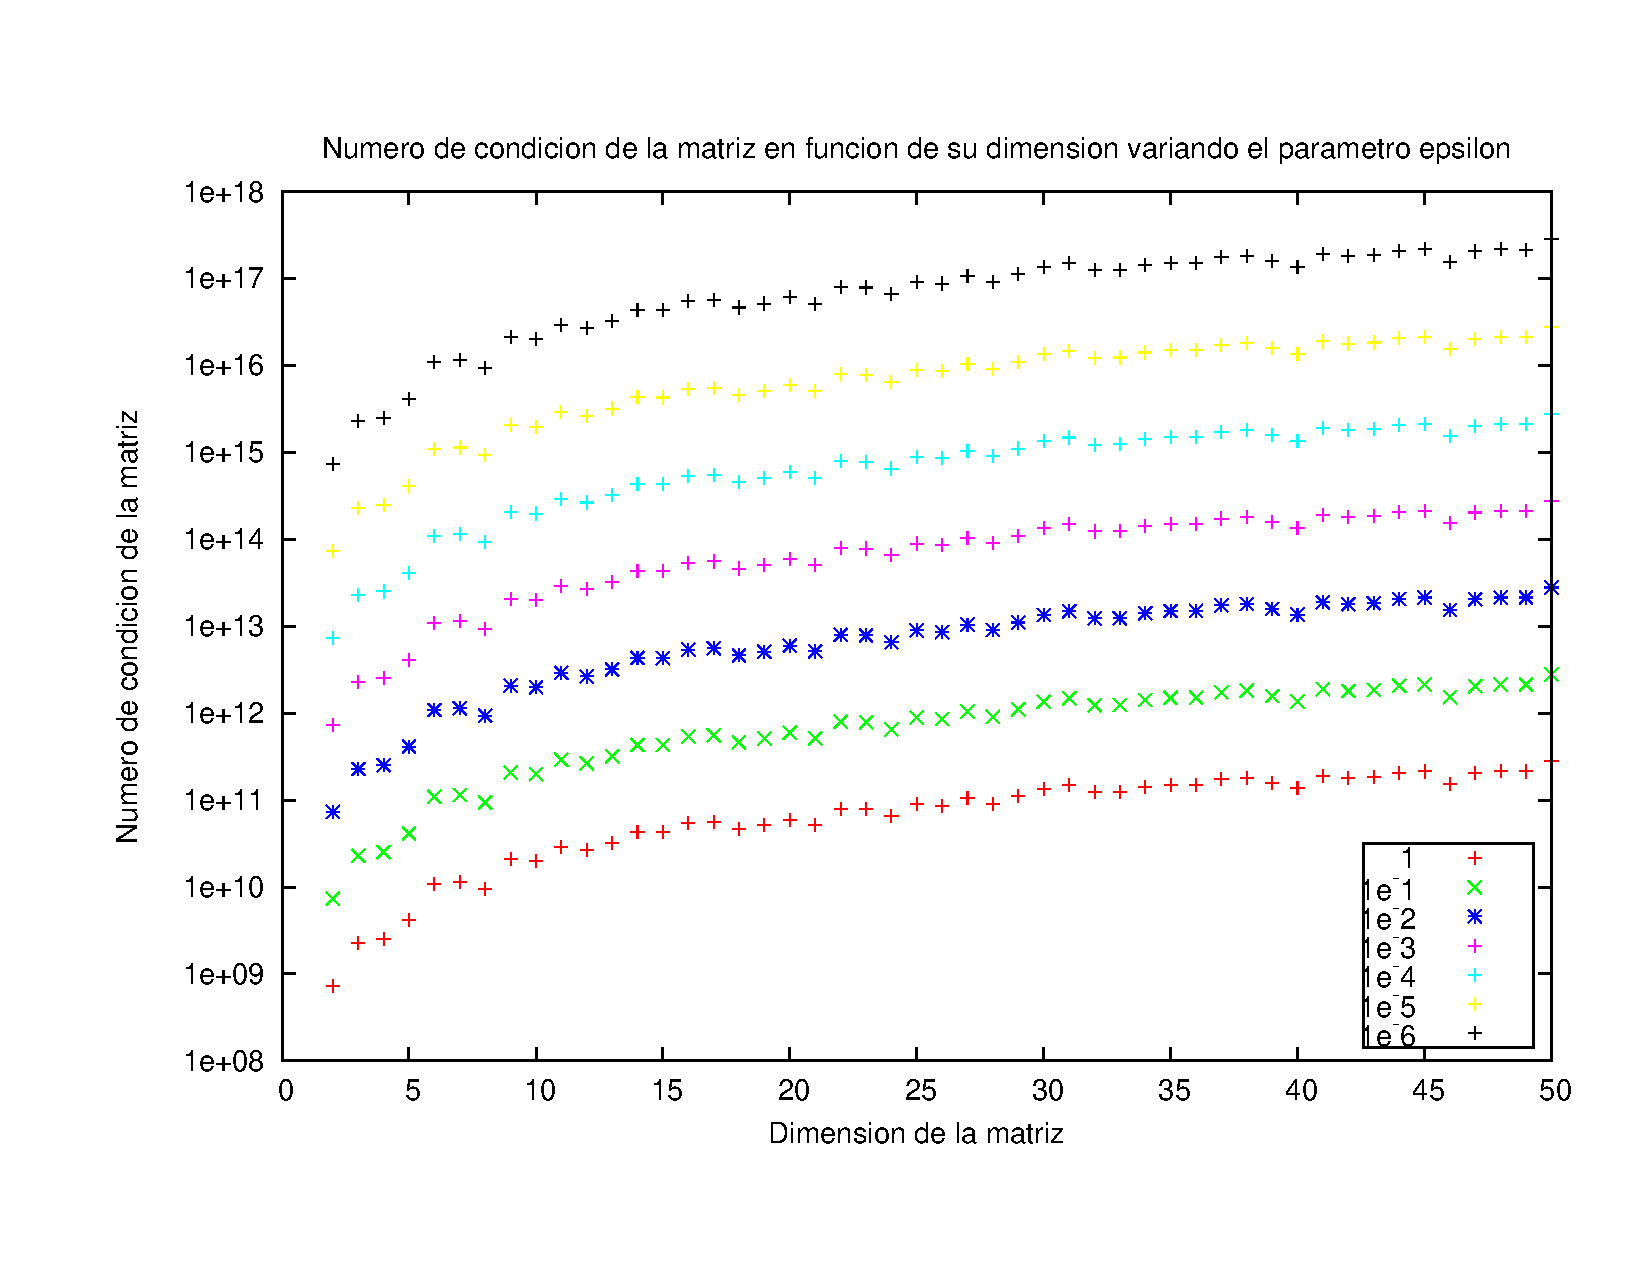
\includegraphics[width=14cm]{graficos/ajuste_epsilon.pdf}
	  \caption{Número de condición de la matriz en función de su dimensión variando el parámetro epsilon}
	  \label{fig:epsilon}
	\end{figure}
\end{section}
